\subsubsection{2.1. Mô hình nhúng ngôn ngữ (Sentence Transformer)}
\indent\indent Trong bài toán phát hiện tài khoản giả mạo (Sybil) trên các mạng xã hội phi tập trung như Lens Protocol, việc phân tích nội dung hồ sơ người dùng đóng vai trò then chốt. Các cụm Sybil thường sử dụng các thuật toán sinh văn bản hoặc sao chép nguyên bản tiểu sử, tên hiển thị và thậm chí là tên định danh để tạo ra hàng loạt tài khoản trong thời gian ngắn. Để máy tính có thể nhận diện được sự tương đồng về mặt ngữ nghĩa này, văn bản cần được chuyển đổi thành các vector số thực trong một không gian toán học, nơi các chuỗi ký tự có ý nghĩa giống nhau sẽ có khoảng cách gần nhau về mặt hình học.\vspace{0.3cm}

Mặc dù kiến trúc BERT (Bidirectional Encoder Representations from Transformers) \cite{devlin2019bert} truyền thống đã tạo nên cuộc cách mạng trong xử lý ngôn ngữ tự nhiên (Natural Language Processing - NLP), nhưng nó lại gặp hạn chế về chi phí tính toán khi so sánh độ tương đồng giữa hàng triệu cặp câu. Để tối ưu hóa quá trình này cho mục tiêu phân loại nút trong đồ thị, nghiên cứu ứng dụng Sentence-BERT (SBERT) được đề xuất bởi Reimers và Gurevych \cite{reimers2019sentence}. Đây là một cải tiến dựa trên kiến trúc Siamese networks, cho phép trích xuất các đặc trưng ngữ nghĩa cấp độ câu một cách hiệu quả.\vspace{0.3cm}

\begin{figure}[H]
    \centering
    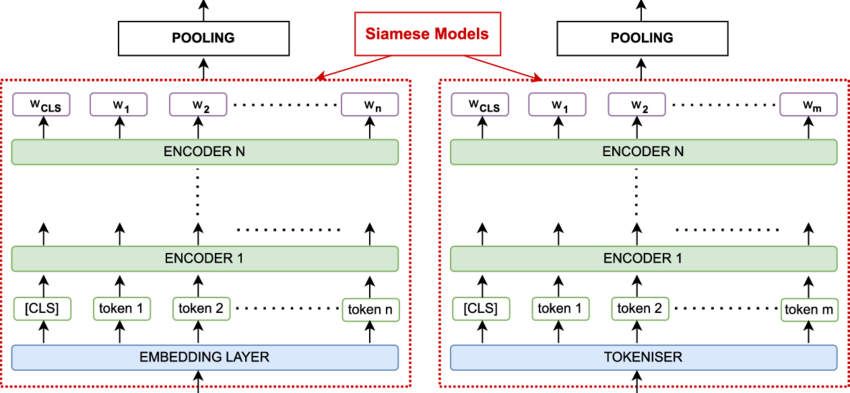
\includegraphics[width=1\linewidth]{images/part-02/chap-01/SBERT.png}
    \vspace{0.5cm}
    \caption{Minh hoạ kiến trúc Siamese của SBERT trong việc trích xuất vector nhúng}
    \label{fig:SBERT}
\end{figure}

Cơ chế trích xuất đặc trưng của SBERT trong hệ thống được vận hành như sau:\vspace{-0.1cm}
\begin{itemize}[label={--}, itemsep=1pt]
    \item \textbf{Siamese Architecture:} Các trường thông tin văn bản (Handle, Display Name, Bio) của tài khoản được đưa qua một mạng Transformer chia sẻ trọng số để tạo ra các vector ngữ cảnh động cho từng từ.
    \item \textbf{Pooling Strategy:} Hệ thống áp dụng chiến lược Mean Pooling để tính trung bình các vector đầu ra của các từ, tạo thành một vector đại diện cố định duy nhất cho toàn bộ thông tin hồ sơ của một tài khoản (\textit{profile embedding}).
    \item \textbf{Semantic Mapping:} Thông qua quá trình này, các tài khoản có hành vi sao chép hồ sơ hoặc sử dụng các mẫu tên định danh tương đồng sẽ được ánh xạ vào các vùng lân cận trong không gian vector, tạo tín hiệu quan trọng cho tầng Similarity của đồ thị.
\end{itemize}

Trong đề tài này, để đảm bảo tốc độ xử lý cho đồ thị quy mô lớn mà vẫn giữ được độ chính xác cao, mô hình \texttt{all-MiniLM-L6-v2} được lựa chọn làm bộ trích xuất đặc trưng văn bản cốt lõi. Mô hình này sở hữu các đặc tính kỹ thuật ưu việt:\vspace{-0.1cm}
\begin{itemize}[label={--}, itemsep=1pt]
    \item \textbf{Kỹ thuật chưng cất tri thức:} Sử dụng kiến trúc MiniLM, đóng vai trò là mô hình "học sinh" được huấn luyện để mô phỏng lại các mối quan hệ self-attention từ các mô hình lớn hơn. Điều này giúp mô hình giữ được khả năng hiểu ngữ cảnh sâu của BERT nhưng với kích thước nhỏ gọn hơn nhiều lần.
    \item \textbf{Hiệu suất vận hành:} Với cấu hình 6 lớp Transformer (L6), mô hình có kích thước chỉ khoảng 80MB, cho tốc độ suy luận nhanh gấp 5 lần so với BERT-base, rất phù hợp để xử lý hàng nghìn nút trên đồ thị mạng xã hội Web3 trong thời gian ngắn.
    \item \textbf{Đặc trưng đầu ra:} Mô hình trích xuất ra một vector nhúng 384 chiều. Đây chính là thành phần chiếm tỷ trọng lớn nhất trong ma trận đặc trưng nút ($X_{raw}$), kết hợp cùng 12 chiều đặc trưng thống kê và hành vi để tạo thành không gian đặc trưng 396 chiều, cung cấp dữ liệu đầu vào toàn diện cho các tầng GNN ở các giai đoạn tiếp theo.
\end{itemize}